\section{Judas}
\label{met:Judas}

Judas, formerly known as Emerald \cite{projthesis}, is a Julia package we've created for internal use for members at \acrshort{cgf}. Our work started last fall, when we saw a limitation of current applications at \acrshort{cgf} for loading \acrshort{das} data from local servers into programs to be able to process and further analyze these data. We chose to write this package in Julia both due to its high performance, and members' familiarity with similar languages such as MatLab and Python. With Julia, we could draw strengths from its ecosystem and build systems to create an easy-to-use library for members to familiarize themselves with. We did so by starting off with a simple python program, that read multiple \acrshort{hdf5} files storing \acrshort{das} data into dataframes. From here, we parallellized certain parts of the code, and opted to store processed data in memory mapped files instead of loading large matrices into memory. This allowed us to work with more data at the same time, as well as decreasing the overall wall time and memory consumption.  

In this section, we will be looking at what changes has been made ever since, from improvements of existent code, to new methods added and the availability of the library for members at \acrshort{cgf}. \\

\subsection{Overview}

Our product is split into two apis. Those being \texttt{Judas} and \texttt{JudasNET}. Judas is the direct continuation from \cite{projthesis}
The \acrshort{api} that's being created is called \texttt{Judas} (Julia and DAS) and is split in 3 modules as well as a seperate Utils file as shown in \ref{fig:ccuda}

\begin{figure}[!h]
    \centering
    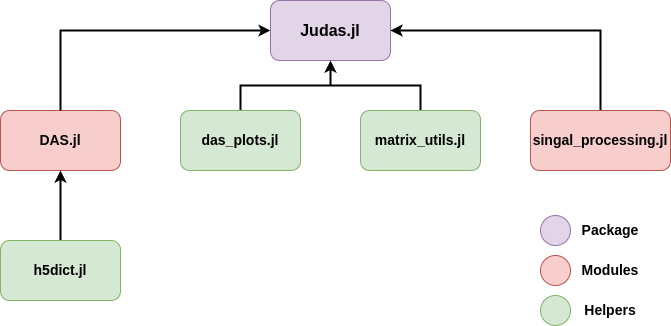
\includegraphics[scale=.6]{figures/judas_overview.png}
    \caption{Overview over our package Judas}
    \label{fig:judasoverview}
\end{figure}


\subsection{Dataset}

Following our previous work, we will be working with data recorded from BANENOR, specifically a train route between Trondheim and Storen with recorded values from the 31st of August 2021 \footnote{Working with national infrastructure requires security clearance, see \ref{app:conf} for more details}. 

\begin{table}[!htbp]
    \centering
    \small
    \begin{tabular}{@{}p{0.3\textwidth}p{0.4\textwidth}p{0.2\textwidth}@{}}
        \toprule
        \textbf{Parameter} & \textbf{Value} & \textbf{Unit} \\
        \midrule
        Experiment & 210830\_NTNU\_Bane\_NOR\_GL8De4F2000 & \\
        File timestamp & 2021-08-31 10:00:01 & \\
        Type of data & Phase rate per distance & rad/m/s \\
        Sampling frequency & 2000.0 & \si{\hertz} \\
        Channel distance & 4.0852 & \si{\meter} \\
        \midrule
        Data shape & 20000 samples \(\times\) 12500 channels & \\
        \midrule
        Gauge length & 8.170401526197452 & \si{\meter} \\
        Sensitivities & 9.362208901094029e6 & r \\
        Regions of interest (ROI) & 1:4:49996 & \\
        \bottomrule
    \end{tabular}
    \caption{BANENOR Experiment Data Summary}
    \label{tab:experiment_data}
\end{table}

As we can see in table \ref{tab:experiment_data}, the total distance of this dataset is approximately 50km, where we have stored data for every 4th sensor across the route. Each file contains 10 seconds of data, leading us to get a matrix of size $20000 x 12500$, where each element is of type \texttt{Float32}, giving us a total of 8GB to be stored for every 10 seconds. This obviously is challenging to work with, so we will go further in depth on how we use resampling and channel decimation to be able to reduce memory usage yet still retain the most important aspects of our signal data. \\


To best showcase what changes and improvements have been made, \ref{fig:apiflow} visualizes the order of high level operations to done on our data. In addition, we will be demonstrating mostly the new additions to the code, as well as the changes to the loading and preprocessing of the data. \\

\begin{figure}[!h]
    \centering
    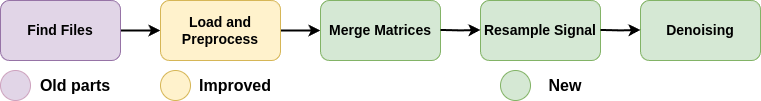
\includegraphics[scale=0.5]{figures/dataflow.png}
    \caption{Dataflow from we read HDF5 files to we are ready to train}
    \label{fig:apiflow}
\end{figure}

\subsection{Pre processing functions}

\subsubsection{Loading \acrshort{das} data}

The \acrshort{das} folder structure has remained largely unchanged. The primary modification involves our data storage approach. Previously, we wrote matrix data to a single large binary file. Now, this data is distributed across multiple files, which are only accessed when specific information is required. This new method optimizes data retrieval and storage efficiency.

Contrary to what was mentioned before, the output of the function \texttt{load\_DAS\_files} has actually changed. Previously, we stored a whole vector of the timestamps for each sample. Not only was this cistly, but actaully totally redundant. If the timestamp of the first row is known, the sampling rate $T$ and which row to look at, one can instead calculate the timestamp like this: 
\lstinline|start_time + MilliSecond(idx * T * 1000)|. This in-place calculation can be done multiple times effectively in Julia using the broadcast operator (.). This ensures that we don't lose essential information before running our data through through the autoencoder

\begin{figure}[!h]
\centering
\begin{subfigure}{.45\textwidth}
  \centering
  \lstinputlisting[language=Julia]{code/dasstructold.jl}
  \caption{Old DAS Struct}
  \label{fig:olddasstc}
\end{subfigure}%
\hfill
\begin{subfigure}{.45\textwidth}
  \centering
  \lstinputlisting[language=Julia]{code/dasstruct.jl}
  \caption{New Layout for DAS struct}
  \label{fig:newdasstc}
\end{subfigure}
\caption{Comparison between different versions of the DAS struct}
\label{fig:dasstccmp}
\end{figure}

From our work on \texttt{Emerald.jl}, the \texttt{find\_DAS\_files} can not be improved much further. 

\lstinputlisting[caption=Parallel processing of \acrshort{das} signal matrices, language=Julia]{code/load_das_files.jl}

\subsubsection{Parallel Resampling}

One of the ways we're able to reduce memory consumption of our program is to resample the signal matrix. What we want to do, is to resample by each sensor, and then combining the results into a new resampled matrix. As we've seen, the original frequency is $2000Hz$, but we want to resample down to $100Hz$, thus only storing $5\%$ of the original data. The following code below shows the implementation of our \texttt{parallel\_resample} function. \\

\lstinputlisting[caption=Implementation of parallel resampling, language=Julia]{code/parallel_resample.jl}

Our parallel resampling approach optimizes performance through memory management and parallel processing techniques. The algorithm proceeds as follows:

\begin{enumerate}
    \item \textbf{Memory Preallocation}: We begin by preallocationg the resultant matrix. This is crucial for performance, as it avoids dynamic memory allocations during the resampling process.
    \item \textbf{Parallel Processing}: We utilize the \texttt{pmap} function from the \texttt{Distributed.jl} package to distribute the resampling workload across multiple processes. Each process is assigned a subset of columns from the input data, allowing for parallel resampling of multiple channels.
    \item \textbf{Resampling}: Within each process, we apply the \texttt{resample} function (from \texttt{DSP.jl}) to individual colums, resampling each channel independently.
    \item \textbf{Data Collection}: To gather the results from the processes, we employ an optimized loop structure. The \texttt{@inbounds} macro disables bounds checking, eliminatin the overhead of boundary checks during array checks. The \texttt{@simd} macro is applied to hint to the compiler to allow for loop reordering, potentially enabling vectorization.
\end{enumerate}


\begin{enumerate}
    \item Judas now make use of multiple processors contra multithreading, seeing major speedups.
    \item Function \texttt{load\_DAS\_files} now writes processed data to a single file back.
\end{enumerate}



\subsubsection{Denoising \acrshort{das} signals}

\lstinputlisting[caption=Denoise function, language=Julia]{code/denoise.jl}

The last addition to \texttt{Judas.jl} is the \texttt{denoise} function. It combines tapering and digital filtering techniques, resulting in an efficient algorithm for \acrshort{das} signal denoising. The function proceeds as follows:

\begin{enumerate}
    \item \textbf{Input validation}: \texttt{denoise} is only performed if tapering is enabled and we are certain the input data is a matrix.
    \item \textbf{Tapering}: A Tukey window (tapered cosine) is applied to mitigate edge effects. Subsequentually, we broadcast the taper across all channels simultaneously.
    \item \textbf{Cutoff Frequency Normalization}: Following, we   normalize the cutoff frequecies by the Nyquist ferquency
    \item \textbf{Digital Filtering}: We utilize the  \texttt{filtfilt} function to apply a zero-phase digital filter, which preserves the phase of the original signal. The filter type provided can be either a lowpass, highpass or a bandpass filter, allowing for selecting approriate filtertype for the scenario. The Butterworth filter design offers a maximally flat frequency response in the passband, providing optimal reduction of noise.
\end{enumerate}

\subsection{General Usage and Distribution}

Our main goal with \texttt{Judas.jl} has been to provide a high performance and easy-to-use library for members at \acrshort{cgf}. To illustrate the ease of use, the following code showcases its simplicity and how users easily can use it alongside other packages. \\

\lstinputlisting[caption=Simple example of how to use Judas, language=Julia]{code/judas_usage.jl}

In addition to the methods we've described in detail, there exist multiple helper methods for plotting and reading/writing \acrshort{das} data. \texttt{Judas.jl} v1.1.0 is currently available for use for members at \acrshort{cgf}. 

\subsection{Evaluation}

In order to evaluate the improvements and additions to this package, we will be performing benchmarks both on individual functions, as well as the overall runtime of a simple usecase. Hereby is a list of different experiments to be conducted:

\begin{itemize}
    \item \textbf{Experiment 1}: Parallel Resample function
    \item \textbf{Experiment 2}: Loading and Processing \acrshort{das} data
\end{itemize}